\documentclass[bigtut]{tutorial}\usepackage[]{graphicx}\usepackage[]{color}
%% maxwidth is the original width if it is less than linewidth
%% otherwise use linewidth (to make sure the graphics do not exceed the margin)
\makeatletter
\def\maxwidth{ %
  \ifdim\Gin@nat@width>\linewidth
    \linewidth
  \else
    \Gin@nat@width
  \fi
}
\makeatother

\definecolor{fgcolor}{rgb}{0.345, 0.345, 0.345}
\newcommand{\hlnum}[1]{\textcolor[rgb]{0.686,0.059,0.569}{#1}}%
\newcommand{\hlstr}[1]{\textcolor[rgb]{0.192,0.494,0.8}{#1}}%
\newcommand{\hlcom}[1]{\textcolor[rgb]{0.678,0.584,0.686}{\textit{#1}}}%
\newcommand{\hlopt}[1]{\textcolor[rgb]{0,0,0}{#1}}%
\newcommand{\hlstd}[1]{\textcolor[rgb]{0.345,0.345,0.345}{#1}}%
\newcommand{\hlkwa}[1]{\textcolor[rgb]{0.161,0.373,0.58}{\textbf{#1}}}%
\newcommand{\hlkwb}[1]{\textcolor[rgb]{0.69,0.353,0.396}{#1}}%
\newcommand{\hlkwc}[1]{\textcolor[rgb]{0.333,0.667,0.333}{#1}}%
\newcommand{\hlkwd}[1]{\textcolor[rgb]{0.737,0.353,0.396}{\textbf{#1}}}%

\usepackage{framed}
\makeatletter
\newenvironment{kframe}{%
 \def\at@end@of@kframe{}%
 \ifinner\ifhmode%
  \def\at@end@of@kframe{\end{minipage}}%
  \begin{minipage}{\columnwidth}%
 \fi\fi%
 \def\FrameCommand##1{\hskip\@totalleftmargin \hskip-\fboxsep
 \colorbox{shadecolor}{##1}\hskip-\fboxsep
     % There is no \\@totalrightmargin, so:
     \hskip-\linewidth \hskip-\@totalleftmargin \hskip\columnwidth}%
 \MakeFramed {\advance\hsize-\width
   \@totalleftmargin\z@ \linewidth\hsize
   \@setminipage}}%
 {\par\unskip\endMakeFramed%
 \at@end@of@kframe}
\makeatother

\definecolor{shadecolor}{rgb}{.97, .97, .97}
\definecolor{messagecolor}{rgb}{0, 0, 0}
\definecolor{warningcolor}{rgb}{1, 0, 1}
\definecolor{errorcolor}{rgb}{1, 0, 0}
\newenvironment{knitrout}{}{} % an empty environment to be redefined in TeX

\usepackage{alltt}
\unitcode{MATH1005}
        \unitname{Statistics}
        \semester{Summer/Winter/Semester2}
        %\sheetnumber1
\IfFileExists{upquote.sty}{\usepackage{upquote}}{}
\begin{document}
\lettersfirst

\begin{tutorial}

\begin{displaybox}
This self-study tutorial is an introduction to R. \\
It should be completed at home before your first tutorial lab.\\
\end{displaybox}
\vskip -2mm

\vspace{.5cm}
{\bf Why learn R/R Studio?}   

Throughout MATH1005 we use a versatile statistical language called {\bf R}, which provides a wide and ever-increasing suite of statistical and graphical techiques. 

{\bf R} is a programming language, which means it is not menu-driven. All commands are case sensitive and are written and executed in the console window at the prompt. However, there
are certain tasks which can be implemented through the menus, like installing new packages. 
Data in R are organised as named structures. We will mainly deal with
the simplest such structures: vectors and matrices. They can be numerical data (like
height and weight) or categorical factors (like gender and type of diet). R treats factors and numerical data differently, and can combine them in a “data frame”. Each vector must contain elements of only one type, while a data frame can contain columns of different types. 

{\bf R Studio} is an integrated user interface for R.  When you open up R Studio, it automatically runs R.

\vspace{.5cm}
\begin{questions}

\question Overview of R  \\

To get an overview of how R works, complete this excellent free online tutorial: tryr.codeschool.com/ \\ 
It takes about an hour but will give you an excellent introduction to R. \\

Another good sumamry is: https://learnxinyminutes.com/docs/r/

\question Download R/R Studio for home usage (free)  \\

R and R Studio are available in the Carslaw computer labs. However we recommend you download both R and R Studio onto your home computer so that you can do your Reports at home, and for use in other subjects. \\

$\bullet$ Download R from the CRAN
(Comprehensive R Archive Network) website:  \\
PC: cran.r-project.org/bin/windows/base/ \\
Mac: cran.r-project.org/bin/macosx/ \\

$\bullet$ Download RStudio: crstudio.com/products/rstudio/download/  \\

Alternatively, you can use RFiddle: http://www.r-fiddle.org/ 

\newpage
\question The layout of R Studio \\

Type commands into the main console window.
Note the `Help' Tab which allows you to look up commands. \\

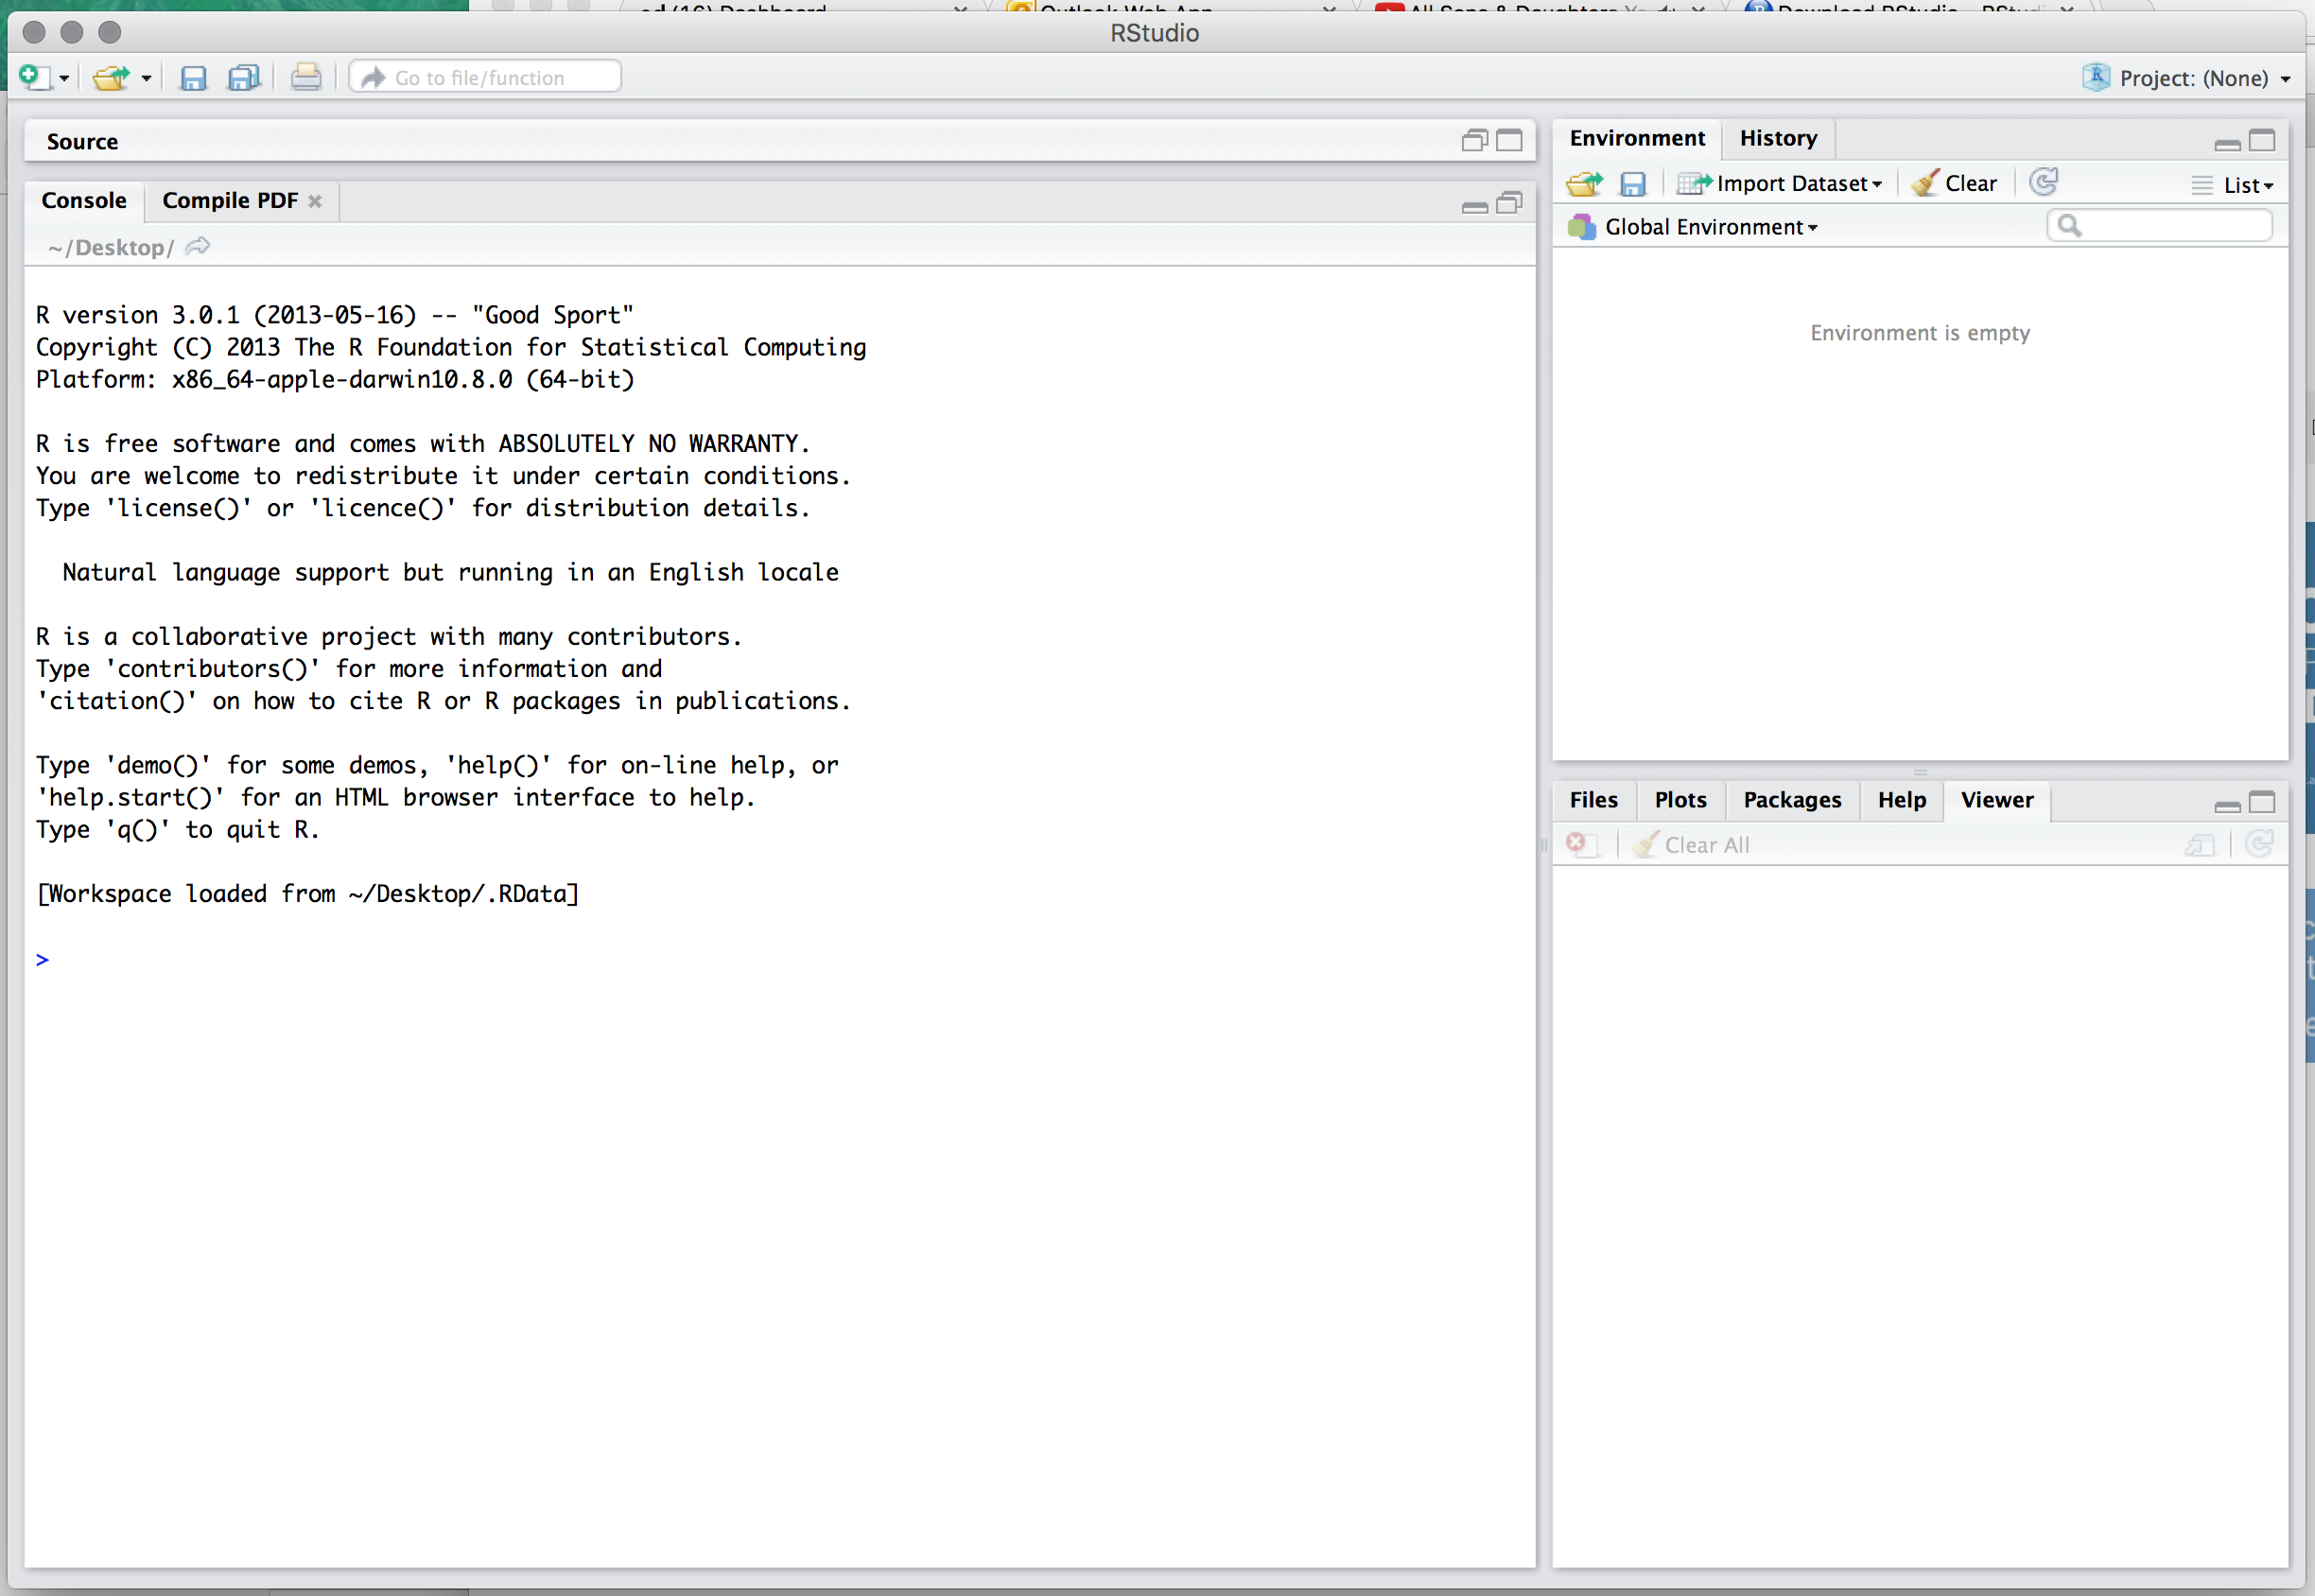
\includegraphics[height=3cm]{RStudioLayout.jpg}

\question Uploading data into RStudio \\

There are many ways to upload data into RStudio, depending on the size of the data and in what form it is stored.

\vspace{1cm}
{\bf Method1: Enter data manually (for small datasets)}

\begin{knitrout}
\definecolor{shadecolor}{rgb}{0.969, 0.969, 0.969}\color{fgcolor}\begin{kframe}
\begin{alltt}
\hlstd{x}\hlkwb{=}\hlkwd{c}\hlstd{(}\hlnum{1.1}\hlstd{,}\hlnum{2.3}\hlstd{,}\hlnum{4.5}\hlstd{,}\hlnum{6.7}\hlstd{,}\hlnum{3.2}\hlstd{)}
\end{alltt}
\end{kframe}
\end{knitrout}

Note that the vector \texttt{x} is now listed in the Environment. \\

To see what is stored inside \texttt{x}, type the name of the vector
\begin{knitrout}
\definecolor{shadecolor}{rgb}{0.969, 0.969, 0.969}\color{fgcolor}\begin{kframe}
\begin{alltt}
\hlstd{x}
\end{alltt}
\begin{verbatim}
## [1] 1.1 2.3 4.5 6.7 3.2
\end{verbatim}
\end{kframe}
\end{knitrout}

\vspace{1cm}
{\bf Method2: Copy and paste the data from a file}

\begin{itemize}
\item At the R prompt enter  \texttt{y=scan()} (the prompt changes to ``\texttt{1:}'' indicating that it is waiting for the 1st data point).
\begin{knitrout}
\definecolor{shadecolor}{rgb}{0.969, 0.969, 0.969}\color{fgcolor}\begin{kframe}
\begin{alltt}
\hlstd{y}\hlkwb{=}\hlkwd{scan}\hlstd{()}
\end{alltt}
\end{kframe}
\end{knitrout}

\vspace{.5cm}
\item Right click to copy and paste these numbers: 1 3 5 7 8 8 

\vspace{.5cm}
\item Click next to the ``\texttt{1:}'' prompt, paste the numbers and hit \textsf{Enter} twice.
\end{itemize}


\vspace{1cm}
{\bf Method3: Import data from the Internet} 

\begin{itemize}
\item
For \texttt{.csv} file: 
\begin{knitrout}
\definecolor{shadecolor}{rgb}{0.969, 0.969, 0.969}\color{fgcolor}\begin{kframe}
\begin{alltt}
\hlstd{Road} \hlkwb{<-} \hlkwd{read.csv}\hlstd{(}\hlstr{"http://www.maths.usyd.edu.au/u/UG/JM/MATH1005/r/StatsData/
                 2016Fatalities.csv"}\hlstd{)}
\end{alltt}
\end{kframe}
\end{knitrout}

\vspace{.5cm}
\item
For \texttt{.txt} file: 
\begin{knitrout}
\definecolor{shadecolor}{rgb}{0.969, 0.969, 0.969}\color{fgcolor}\begin{kframe}
\begin{alltt}
\hlstd{Mice} \hlkwb{<-} \hlkwd{read.table}\hlstd{(}\hlstr{"http://www.maths.usyd.edu.au/u/UG/JM/MATH1005/r/StatsData/Mice.txt"}\hlstd{)}
\end{alltt}
\end{kframe}
\end{knitrout}

\begin{knitrout}
\definecolor{shadecolor}{rgb}{0.969, 0.969, 0.969}\color{fgcolor}\begin{kframe}
\begin{alltt}
\hlstd{Mice}\hlkwb{=}\hlkwd{scan}\hlstd{(}\hlkwc{file}\hlstd{=}\hlkwd{url}\hlstd{(}\hlstr{"www.maths.usyd.edu.au/u/UG/JM/MATH1005/r/StatsData/Mice.txt"}\hlstd{))}
\end{alltt}
\end{kframe}
\end{knitrout}

\end{itemize}

\newpage

{\bf Method4: Import a file from a directory} \\

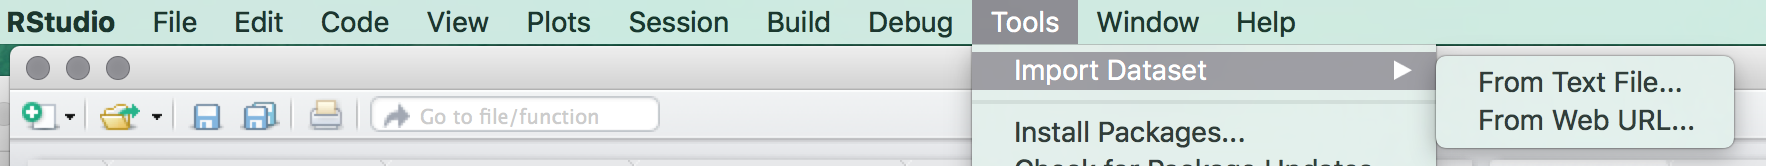
\includegraphics[height=1.5cm]{ImportData.jpg}


\vspace{1cm}
{\bf Method5: Import a file from a directory}

\begin{itemize}

\item
Download the {\tt 2016Fatalities.csv} file into a directory. \\
The data files are found here: 
http://www.maths.usyd.edu.au/u/UG/JM/StatsData.html \\

\item
Change the RStudio Working Directory to where your file is stored, by clicking on \textsf{Session/Set Working Directory/Choose Directory} and choosing where the file is stored. \\

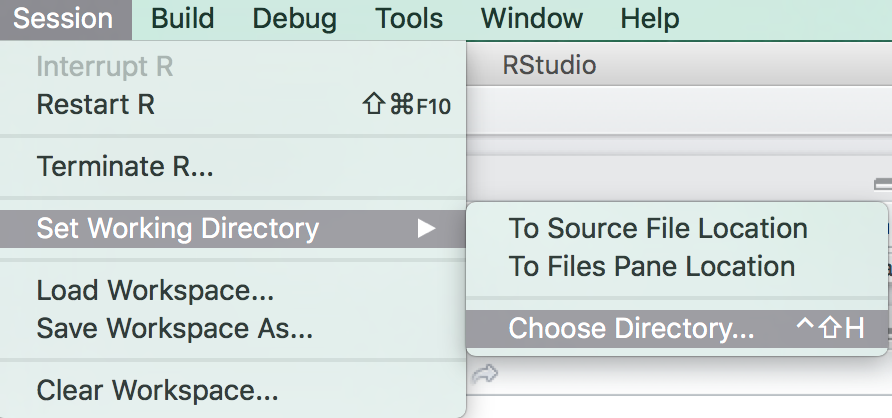
\includegraphics[height=3.5cm]{Setwd.jpg} \\

\item
Alternatively, use the command 
\begin{knitrout}
\definecolor{shadecolor}{rgb}{0.969, 0.969, 0.969}\color{fgcolor}\begin{kframe}
\begin{alltt}
\hlkwd{setwd}\hlstd{()}
\end{alltt}
\end{kframe}
\end{knitrout}
to specify the directoryaddress. \\

\item
Upload the file into R.

\begin{knitrout}
\definecolor{shadecolor}{rgb}{0.969, 0.969, 0.969}\color{fgcolor}\begin{kframe}
\begin{alltt}
\hlstd{Road} \hlkwb{<-} \hlkwd{read.csv}\hlstd{(}\hlstr{"2016Fatalities.csv"}\hlstd{,}\hlkwc{header}\hlstd{=T)}
\end{alltt}
\end{kframe}
\end{knitrout}

\vspace{.5cm}
Note: You can check what the Working Directory is by using 
\begin{knitrout}
\definecolor{shadecolor}{rgb}{0.969, 0.969, 0.969}\color{fgcolor}\begin{kframe}
\begin{alltt}
\hlkwd{getwd}\hlstd{()}
\end{alltt}
\end{kframe}
\end{knitrout}
\end{itemize}



\question Snapshot of Multivariate Data \\

\begin{itemize}

\item
The \texttt{dim} command gives the dimension of the matrix.
\begin{knitrout}
\definecolor{shadecolor}{rgb}{0.969, 0.969, 0.969}\color{fgcolor}\begin{kframe}
\begin{alltt}
\hlkwd{dim}\hlstd{(Road)}
\end{alltt}
\begin{verbatim}
## [1] 442  18
\end{verbatim}
\end{kframe}
\end{knitrout}

\vspace{.5cm}
\item
The \texttt{names} command lists the variables.
\begin{knitrout}
\definecolor{shadecolor}{rgb}{0.969, 0.969, 0.969}\color{fgcolor}\begin{kframe}
\begin{alltt}
\hlkwd{names}\hlstd{(Road)}
\end{alltt}
\begin{verbatim}
##  [1] "Crash.ID"                        "State"                          
##  [3] "Date"                            "Day"                            
##  [5] "Month"                           "Year"                           
##  [7] "Dayweek"                         "Time"                           
##  [9] "Hour"                            "Min"                            
## [11] "Crash.Type"                      "BusInvolvement"                 
## [13] "RigidTruck..Involvement"         "Articulated.Truck..Involvement."
## [15] "SpeedLimit"                      "RoadUser"                       
## [17] "Gender"                          "Age"
\end{verbatim}
\end{kframe}
\end{knitrout}

\vspace{.5cm}
\item
The \texttt{head} command lists the top of the dataset, where \texttt{1} specifies the 1st row.
\begin{knitrout}
\definecolor{shadecolor}{rgb}{0.969, 0.969, 0.969}\color{fgcolor}\begin{kframe}
\begin{alltt}
\hlkwd{head}\hlstd{(Road,}\hlnum{1}\hlstd{)}
\end{alltt}
\begin{verbatim}
##     Crash.ID State     Date Day   Month Year Dayweek  Time Hour Min
## 1 2.2016e+12   VIC 1-Jan-16   1 January 2016  Friday 20:30   20  30
##       Crash.Type BusInvolvement RigidTruck..Involvement
## 1 Single vehicle             No                      No
##   Articulated.Truck..Involvement. SpeedLimit         RoadUser Gender Age
## 1                              No         80 Motorcycle rider   Male  25
\end{verbatim}
\end{kframe}
\end{knitrout}

\vspace{.5cm}
\item
The \texttt{str} command classifies each variable.
{\tiny 
\begin{knitrout}
\definecolor{shadecolor}{rgb}{0.969, 0.969, 0.969}\color{fgcolor}\begin{kframe}
\begin{alltt}
\hlkwd{str}\hlstd{(Road)}
\end{alltt}
\begin{verbatim}
## 'data.frame':	442 obs. of  18 variables:
##  $ Crash.ID                       : num  2.2e+12 4.2e+12 1.2e+12 5.2e+12 6.2e+12 ...
##  $ State                          : Factor w/ 8 levels "ACT","NSW","NT",..: 7 5 2 8 6 6 4 6 2 2 ...
##  $ Date                           : Factor w/ 113 levels "1-Apr-16","1-Feb-16",..: 3 3 44 44 44 44 86 86 95 95 ...
##  $ Day                            : int  1 1 2 2 2 2 3 3 4 4 ...
##  $ Month                          : Factor w/ 4 levels "April","February",..: 3 3 3 3 3 3 3 3 3 3 ...
##  $ Year                           : int  2016 2016 2016 2016 2016 2016 2016 2016 2016 2016 ...
##  $ Dayweek                        : Factor w/ 7 levels "Friday","Monday",..: 1 1 3 3 3 3 4 4 2 2 ...
##  $ Time                           : Factor w/ 225 levels "0:00","0:12",..: 150 10 5 109 135 135 64 37 149 164 ...
##  $ Hour                           : int  20 1 0 17 19 19 14 11 20 21 ...
##  $ Min                            : int  30 0 30 20 58 58 0 55 25 45 ...
##  $ Crash.Type                     : Factor w/ 3 levels "Multiple vehicle",..: 3 3 3 1 1 1 2 1 3 3 ...
##  $ BusInvolvement                 : Factor w/ 2 levels "No","Yes": 1 1 1 1 1 1 1 1 1 1 ...
##  $ RigidTruck..Involvement        : Factor w/ 2 levels "No","Yes": 1 1 1 1 1 1 1 1 1 1 ...
##  $ Articulated.Truck..Involvement.: Factor w/ 2 levels "No","Yes": 1 1 1 2 1 1 1 1 1 1 ...
##  $ SpeedLimit                     : int  80 110 100 110 80 80 60 100 100 60 ...
##  $ RoadUser                       : Factor w/ 6 levels "Bicyclist (includes pillion passengers)",..: 4 2 5 2 4 3 6 4 2 2 ...
##  $ Gender                         : Factor w/ 2 levels "Female","Male": 2 2 2 2 2 2 2 2 2 1 ...
##  $ Age                            : int  25 40 18 53 17 31 70 51 59 17 ...
\end{verbatim}
\end{kframe}
\end{knitrout}
}

\vspace{.5cm}
\item
To choose a particular variable, select \texttt{dataname\$variablename}
\begin{knitrout}
\definecolor{shadecolor}{rgb}{0.969, 0.969, 0.969}\color{fgcolor}\begin{kframe}
\begin{alltt}
\hlstd{SpeedLimit} \hlkwb{<-} \hlstd{Road}\hlopt{$}\hlstd{SpeedLimit}
\end{alltt}
\end{kframe}
\end{knitrout}


\vspace{.5cm}
\item
To classify a particular variable, use the \texttt{class} command.
\begin{knitrout}
\definecolor{shadecolor}{rgb}{0.969, 0.969, 0.969}\color{fgcolor}\begin{kframe}
\begin{alltt}
\hlkwd{class}\hlstd{(SpeedLimit)}
\end{alltt}
\begin{verbatim}
## [1] "integer"
\end{verbatim}
\end{kframe}
\end{knitrout}

\vspace{.5cm}
\item
A factor can be re-classified as numerical by using the \texttt{as.numeric} command.

\vspace{.5cm}
\item
Most commands are easy to guess.
\begin{knitrout}
\definecolor{shadecolor}{rgb}{0.969, 0.969, 0.969}\color{fgcolor}\begin{kframe}
\begin{alltt}
\hlkwd{mean}\hlstd{(SpeedLimit)}
\hlkwd{hist}\hlstd{(SpeedLimit)}
\hlstd{x}\hlopt{+}\hlnum{1}
\hlnum{1}\hlopt{/}\hlnum{2}\hlopt{*}\hlstd{(}\hlkwd{exp}\hlstd{(x))}
\end{alltt}
\end{kframe}
\end{knitrout}


\end{itemize}

\question Saving Results \\

It is good practise to make a summary of your work in each tutorial. The easiest way is to: \\
(1) Open an RScript file [Click on \textsf{File/New File/R Script}] \\
(2) Copy and paste useful commands. \\
(3) Save the file. \\
(4) In RStudio, you can reopen this file at any time, and press \textsf{Run} to perform the commands again. \\

\end{questions}
\end{tutorial}
\end{document}

